\subsection{ROOT Analysis}

The binary data from the DAQ acquisition was analyzed through a C++ code
implemented in a ROOT framework~\cite{root}.

\bigbreak

The Pulse Shape Analysis (PSA) were performed directly on the binary data, as,
by doing thus, it is not necessary to save the signal pulse as a ROOT variable
and a further analysis can be facilitated. The \num{100} ns long stamps of the
signal, saved by the digitizer, were used to obtain two discriminating
variables, that describe fully the important features of the pulse signal for
the proton and $\alpha$ identification: $\tau _{\textup{rise}}$ and
$i_{\textup{max}}$, which represent, respectively, the rise time and maximum
derivative of the signal.

\bigbreak

In order to calulcate the two, the following algorithms were used:

\begin{itemize}

\item For the rise time, $\tau _{\textup{rise}}$, the difference between the moment when the pulse is at
  70\%, $t_{0.7}$, and when it is at 30\%, $t_{0.3}$ is considered.
  In order to calculate it, the maximum value of the signal, $V_{\textup{max}}$,
  was obtained as the mean of 3 highest values found. Then, two nearest points
  to 30\% (and 70\%) of the signal were found, in order to perform a two-point
  linear interpolation. Then the $t_{0.3}$ (and $t_{0.7}$) (Fig. \ref{pulse} is found from the
  interpolating function as the time when the signal height is at
  $0.3 V_{\textup{max}}$
  (and $0.7 V_{\textup{max}}$).
\item For the maximum derivative of the pulse, $i_{\textup{max}}$, 
  the interpolation of the Pulse Shape was performed using a ROOT class,
  called TSpline3, and 5 highest values of its derivative are used for the
  mean value which is the $i_{\textup{max}}$.

\end{itemize}

\begin{figure}[h]
  \centering
  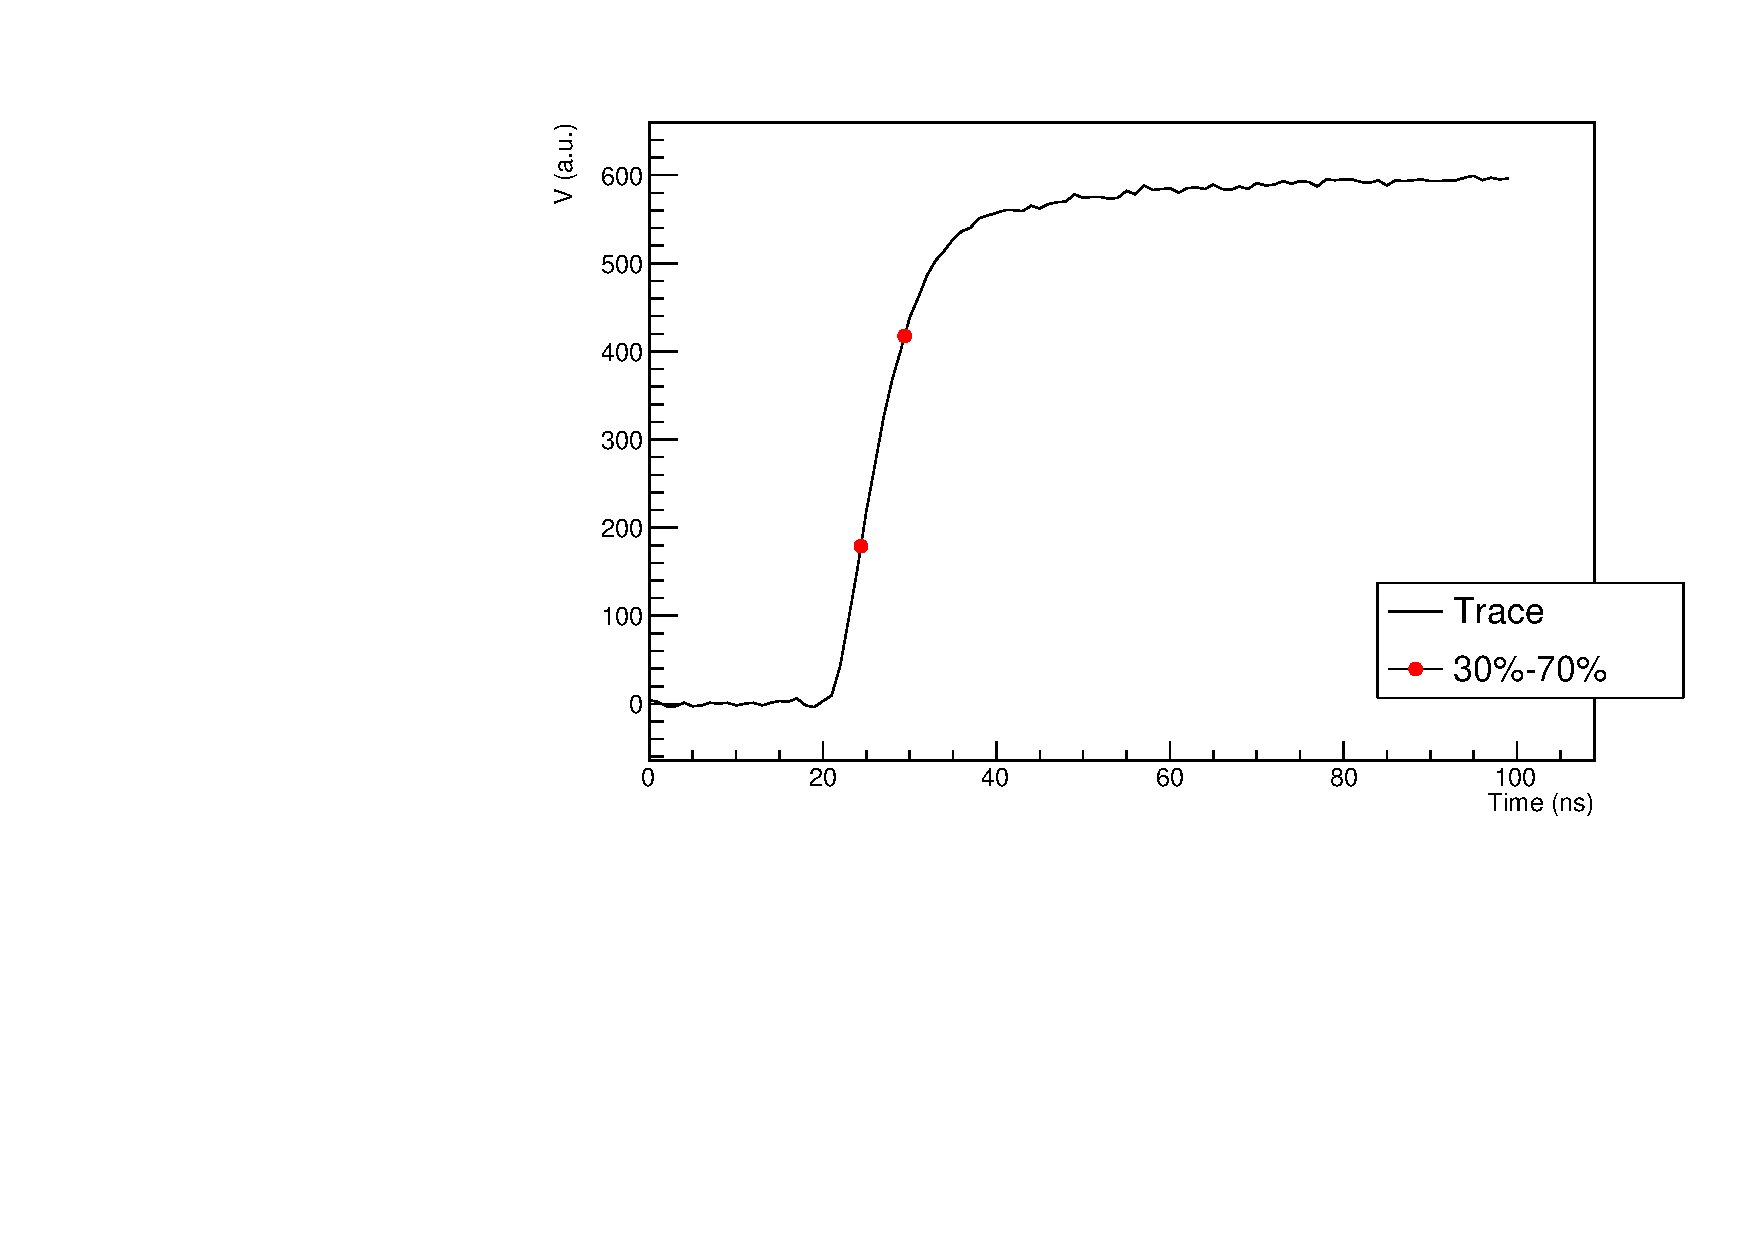
\includegraphics[scale=.6]{img/example_pulse.pdf}
  \caption{An example of the Trace pulse signal. The two points represent the $t_{0.3}$ and $t_{0.7}$.}
  \label{pulse}
\end{figure}

\bigbreak

At the end, for each experimental run and each digitizer (the \textit{gal09}
one, and the \textit{gal10}), a TTree object, called \textit{TraceEvent}, was created with the following variables:

\begin{itemize}
\item fDomain
\item fTimeStamp
\item fSubData (vector)
  \begin{itemize}
  \item fSubDomain
  \item fEnergy
  \item fTrace
  \item fTime
  \item fBaseline
  \item fPSA
  \end{itemize}
\end{itemize}
where \textit{fDomain} is the ID of the DAQ used, \textit{fTimeStamp} is the
time given by the digitizer, \textit{fSubDomain} is the detector channel,
\textit{fEnergy} is the energy of the particle and the others are variables
filled according to the PSA: \textit{fTime} is the calculated rise time and
\textit{fTrace} is the maximum derivative of the signal (\textit{fBaseline} and
\textit{fPSA} were later used as Neural Network outputs that gives the
probability of the particle being either a proton or an alpha).

\bigbreak

Plots of the $\tau _{\textup{rise}}$ and $i_{\textup{max}}$ in function of the energy
are shown in Fig.~\ref{imax} and Fig.~\ref{risetime}. The $\alpha$ and proton
regions are clearly visible and so they can be tagged and used for the
Neural Network construction. Moreover, even though the signal regions seem almost
backgroundless, many pulses are present that can not be tagged as neither a
proton nor $\alpha$. In fact, the protons stop at $\approx 4$ MeV and
$\alpha$'s at $\approx 6$ MeV as expected from detector response simulations
performed through LISE software~\cite{lise} (origins of the remaining signals
are not known).

\begin{figure}[h]
  \centering
  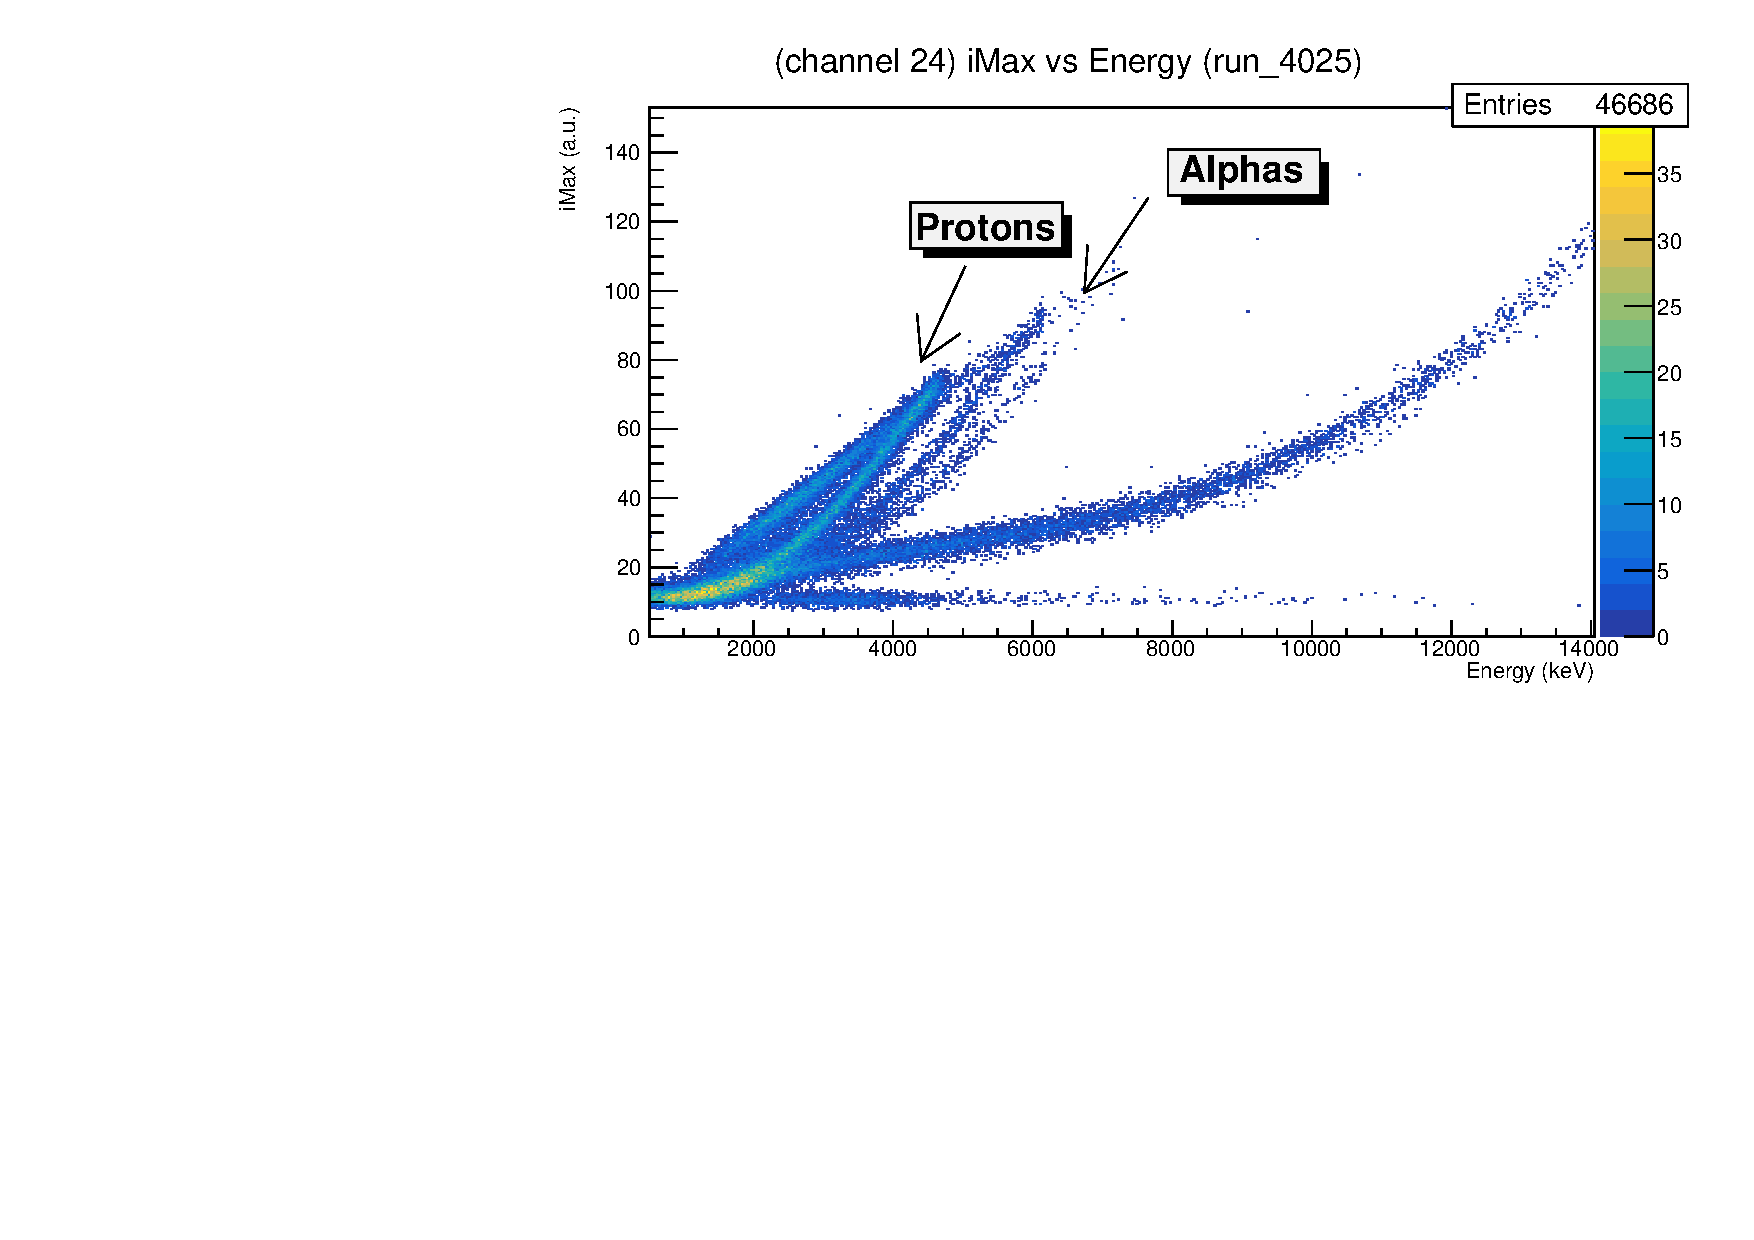
\includegraphics[scale=.6]{img/iMax_4025.pdf}
  \caption{An example of the $i_{\textup{max}}$ vs \textit{E} graph for the 4025 run (only one channel is considered).}
  \label{imax}
\end{figure}

\begin{figure}[h]
  \centering
  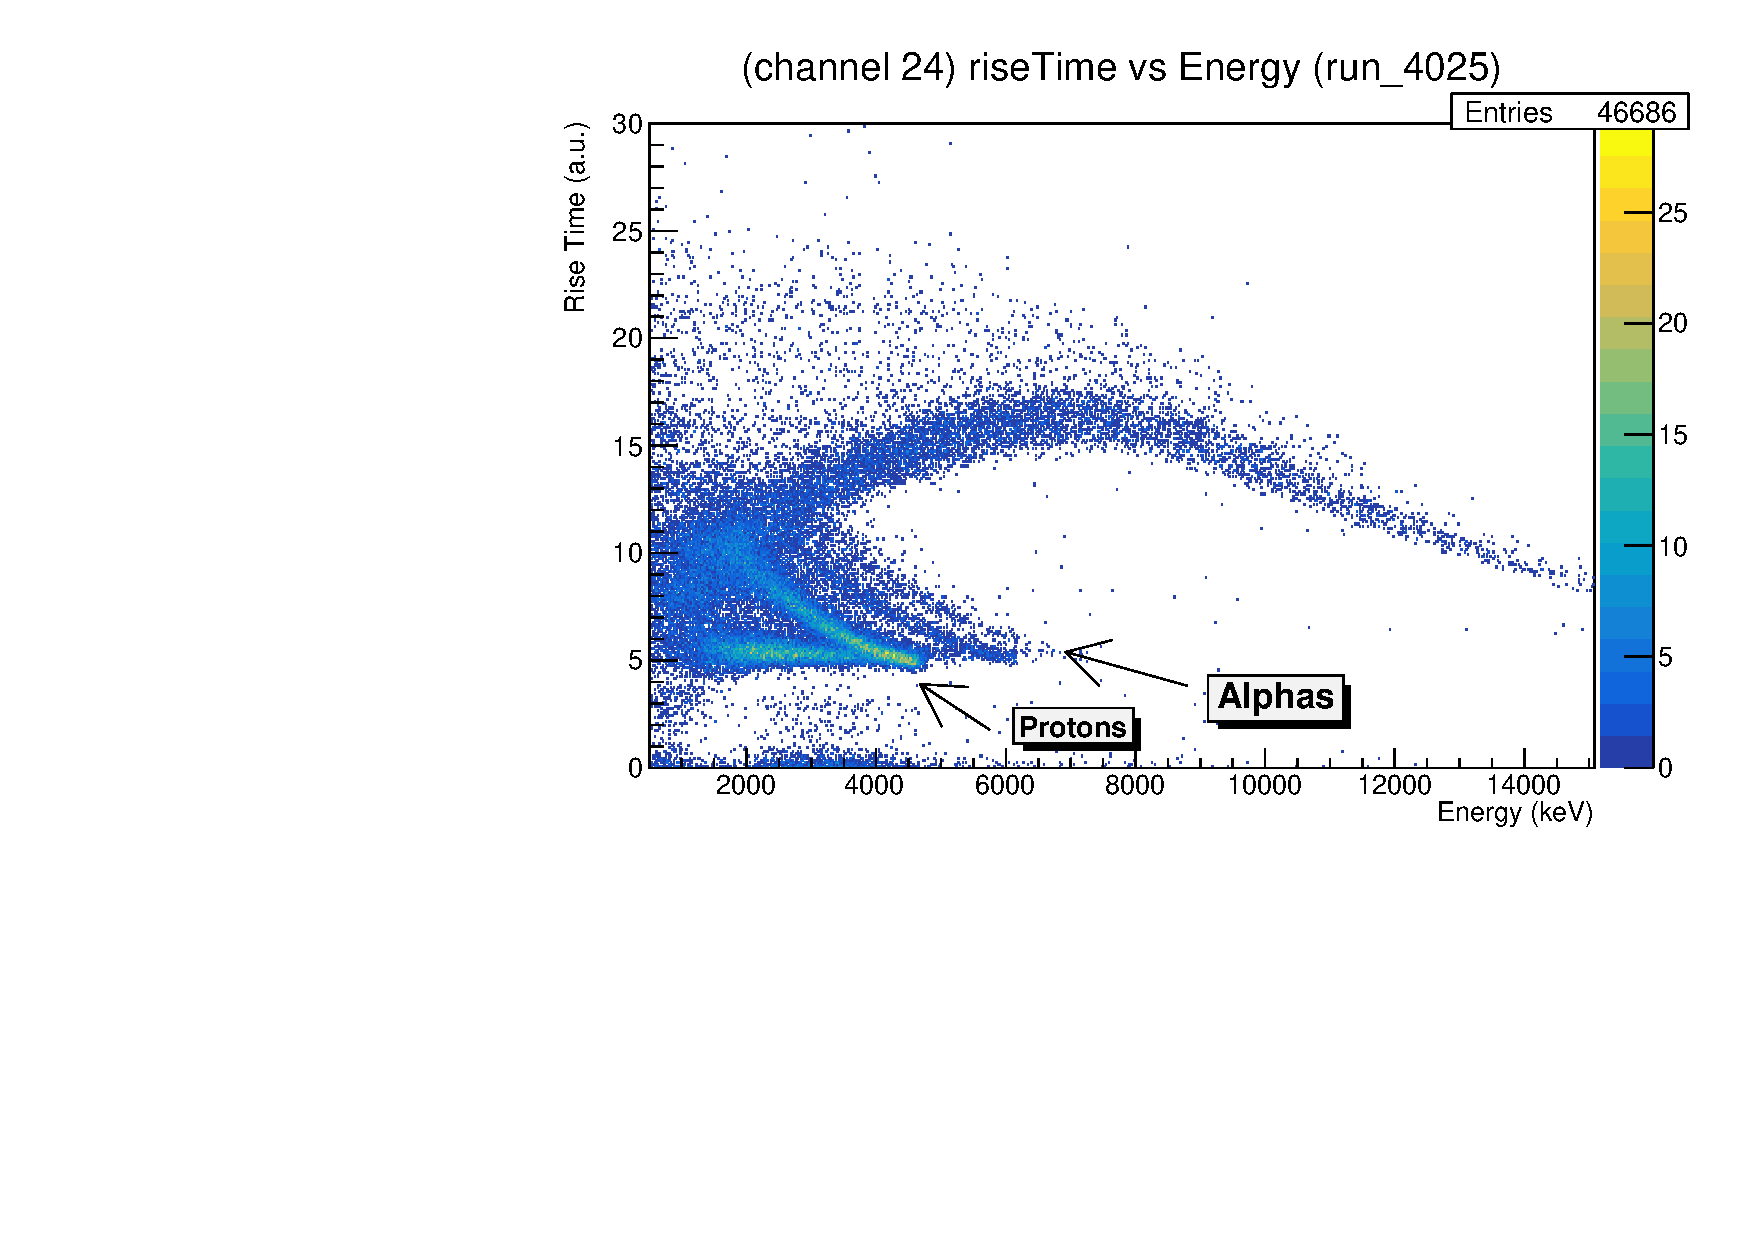
\includegraphics[scale=.6]{img/riseTime_4025.pdf}
  \caption{An example of the $\tau _{\textup{rise}}$ vs \textit{E} graph for the 4025 run (only one channel is considered).}
  \label{risetime}
\end{figure}

\clearpage